\documentclass[compress,red,mathsans,10pt]{beamer}
\usepackage{beamerthemesplit}
\usepackage{amssymb}
\usepackage{multirow}
%\usetheme{Antibes}
\usepackage{pgf,pgfarrows,pgfnodes}

\setbeamercolor{uppercol}{fg=white,bg=purple}%
\setbeamercolor{lowercol}{fg=black,bg=pink}%


\usecolortheme{lily}
\begin{document}
\title{Aplicacions Estad\'{\i}stiques}
\subtitle{Enginyeria Edificaci\'o 2009/10.}  
\author{Antonio E. Teruel}
\date{}

\frame{\titlepage} 

\frame{\frametitle{Temari}
\begin{itemize}
\item \only<1>{Estad\'{\i}stica Descriptiva}
      \only<2->{\color{red}Estad\'{\i}stica Descriptiva\color{black}}
	\begin{itemize}
	\item [] Tema 1. An\`alisi exploratori de dades.
	\item [] Tema 2. Distribucions estad\'{\i}stiques bidimensionals. 
	\end{itemize}
\item Probabilitat.
	\begin{itemize}
	 \item [] Tema 3. Teoria de la probabilitat.
	\end{itemize}
\item Estad\'{\i}stica Inferencial.
	\begin{itemize}
	\item [] Tema 4. Variables aleat\`ories discretes.
	\item [] Tema 5. Variables aleat\`ories continues.
	\item [] Tema 6. Estimaci\'o de par\`ametres.
	\item [] Tema 7. Contrast d'hipòtesis.
	\end{itemize}
\end{itemize}
}

\frame{\frametitle{Estad\'{\i}stica}
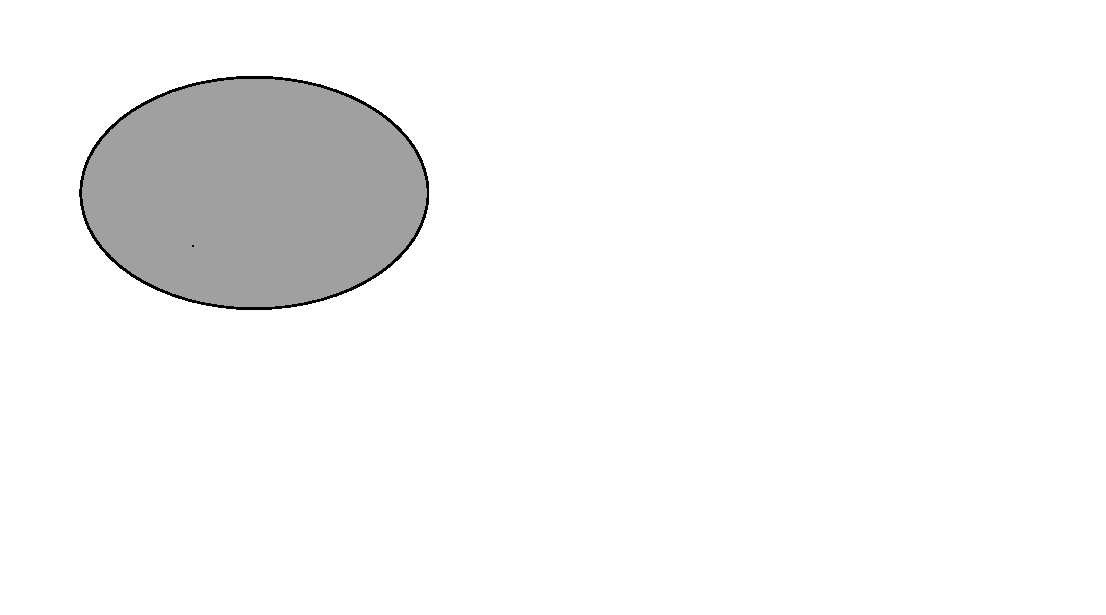
\includegraphics[width=10cm]{Dbes0101.eps}
		\put(-240,105){Poblaci\'o}
		\put(-260,135){$N$}
		\put(-150,135){$X$}
		\put(-110,125){$\mu_{X}, \sigma^2_{X}$}
		\put(-230,65){$n$}
		\put(-240,37){mostra}
		\put(-150,30){$Y$}
		\put(-110,25){$\mu_{Y}, \sigma^2_{Y}$}
		\put(-155,75){Probabilitat}
}

\frame{\frametitle{Estad\'{\i}stica Descriptiva}
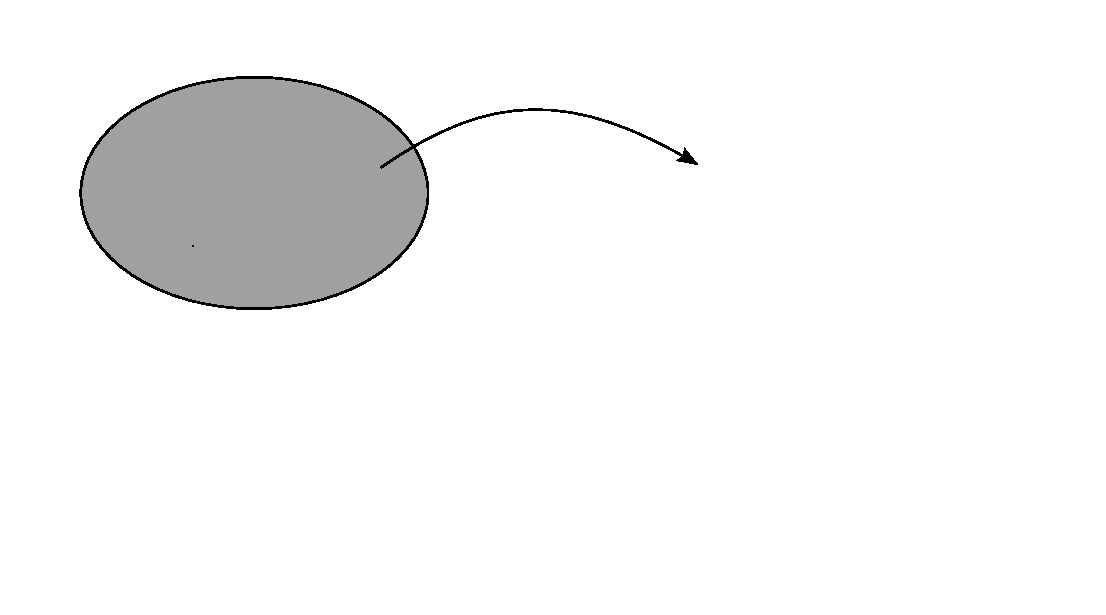
\includegraphics[width=10cm]{Dbes0102.eps}
		\put(-240,105){Poblaci\'o}
		\put(-260,135){$N$}
		\put(-150,135){$X$}
		\put(-110,125){$\mu_{X}, \sigma^2_{X}$}
		\put(-250,65){$n$}
		\put(-240,37){mostra}
		\put(-150,30){$Y$}
		\put(-110,25){$\mu_{Y}, \sigma^2_{Y}$}
		\put(-155,75){Probabilitat}
	
}

\frame{\frametitle{Conceptes B\`asics}
\begin{columns}
\begin{column}{0.5\textwidth}
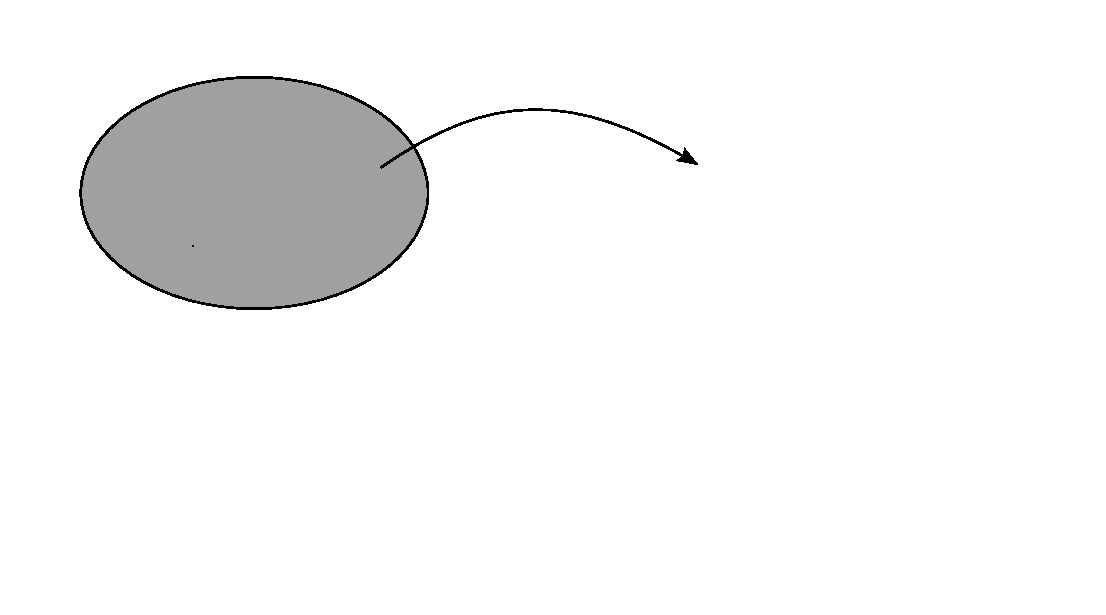
\includegraphics[width=8cm]{Dbes0102.eps}
		\put(-200,90){Poblaci\'o}
		\put(-215,110){$N$}
		\put(-125,110){$X$}
		\put(-90,105){$\mu_{X}, \sigma^2_{X}$}
		\put(-210,50){$n$}
		\put(-235,37){mostra}
		\put(-135,25){$Y$}
		\put(-110,15){$\mu_{Y}, \sigma^2_{Y}$}
		\put(-135,60){Probabilitat}
\end{column}
\begin{column}{0.5\textwidth}
\begin{itemize}
\item \textbf{Est. Descriptiva}: ci\`encia per a la descripci\'o i organitzaci\'o de dades.
\item <2->\textbf{Dades}: unitats d'informaci\'o recopilades durant l'estudi estad\'{\i}stic 
	\begin{itemize}
	\item <3->\textbf{Poblaci\'o}: conjunt total d'individus sobre el qual es fa l'estudi estad\'{\i}stic
	\item <4->\textbf{Mostra}:  subconjunt del conjunt total
	\end{itemize}
\end{itemize}
\end{column}

\end{columns}
}

\frame{\frametitle{Conceptes B\`asics}
\begin{columns}
\begin{column}{0.5\textwidth}
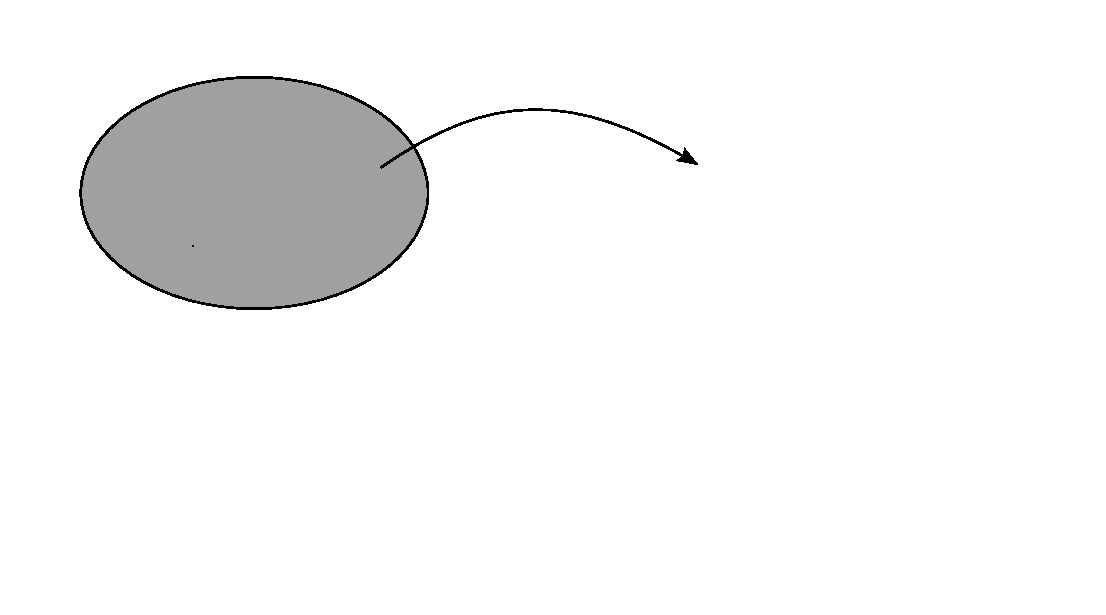
\includegraphics[width=8cm]{Dbes0102.eps}
		\put(-200,90){Poblaci\'o}
		\put(-215,110){$N$}
		\put(-125,110){$X$}
		\put(-90,105){$\mu_{X}, \sigma^2_{X}$}
		\put(-210,50){$n$}
		\put(-235,37){mostra}
		\put(-135,25){$Y$}
		\put(-110,15){$\mu_{Y}, \sigma^2_{Y}$}
		\put(-135,60){Probabilitat}
\end{column}
\begin{column}{0.5\textwidth}
\begin{itemize}
\item \textbf{Est. Descriptiva}: ci\`encia per a la descripci\'o i organitzaci\'o de dades.
\item \textbf{Dades}: unitats d'informaci\'o recopilades durant l'estudi estad\'{\i}stic 
	\begin{itemize}
	\item \textbf{Poblaci\'o}: Per a un estudi sobre la satisfacci\'o dels clients d'un hotel es 		passa un q\"uestionari a tots els clients
	\item \textbf{Mostra}: Per a un estudi sobre el frac\`as escolar a Balears es prenen les dades 		de 5 escoles de Mallorca, 2 de Menorca i 2 d'Eivissa 
	\end{itemize}
\end{itemize}
\end{column}
\end{columns}
}

\frame{\frametitle{Conceptes B\`asics}
\begin{columns}
\begin{column}{0.5\textwidth}
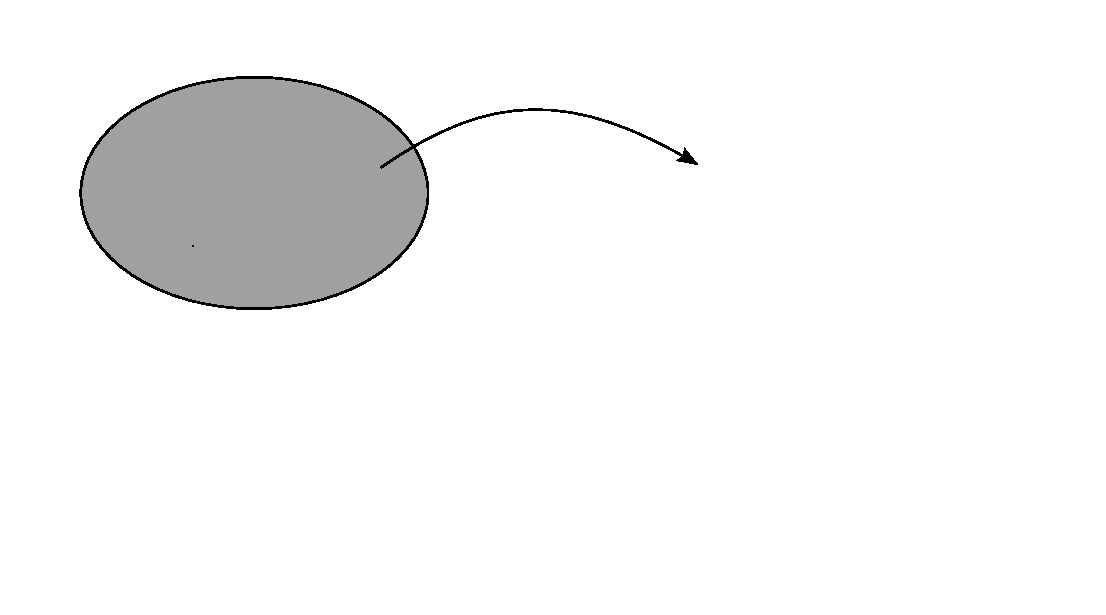
\includegraphics[width=8cm]{Dbes0102.eps}
		\put(-200,90){Poblaci\'o}
		\put(-215,110){$N$}
		\put(-125,110){$X$}
		\put(-90,105){$\mu_{X}, \sigma^2_{X}$}
		\put(-210,50){$n$}
		\put(-235,37){mostra}
		\put(-135,25){$Y$}
		\put(-110,15){$\mu_{Y}, \sigma^2_{Y}$}
		\put(-135,60){Probabilitat}
\end{column}
\begin{column}{0.5\textwidth}
\begin{itemize}
\item \textbf{Variables}:  caracter\'{\i}stiques o atributs dels individus que formen la poblaci\'o i que volem estudiar
\end{itemize}
\end{column}
\end{columns}
}

\frame{\frametitle{Conceptes B\`asics. Classificaci\'o de Variables}
\begin{columns}
\begin{column}{1.1\textwidth} 
\begin{tabular}{|p{2cm}|p{2cm}|p{2cm}|p{4.5cm}|} \hline
   \multirow{4}{*} {Tipus dades} & \multirow{2}{1cm} {Quantitatives: prenen valors num\`erics } & 
		discretas & nombre d'alumnes matriculats d'estadística \\ \cline{3-4}
       	&  & continues & temperatura mesurada per una estaci\'o meteorol\'ogica \\ \cline{2-4}
   				 & \multirow{2}{1cm} {Qualitatives: no prenen valors num\`erics} &
		ordinals: es poden ordenar & grau de satisfacci\'o dels clients d'un hotel (insatisfet, poc satisfet, satisfet, molt satisfet \\ \cline{3-4}
	& & nominals: no es poden ordenar & tipus d'establiment hoteler (hotel rural, hotel de ciutat, hotel de platja)  \\ \hline
  \multirow{2}{*}{Dimensi\'o} & \multicolumn{2}{l|}{Unidimensional} &  al\c{c}ada, edat \\ \cline{2-4}
			& \multicolumn{2}{l|}{Multidimensional} & edat i al\c{c}ada, sexe i pes\\ \hline
  \multirow{2}{*}{Temporalitat} & \multicolumn{2}{l|}{Atemporal} &  pes d'un conjunt de persones, color dels ulls \\ \cline{2-4}
			& \multicolumn{2}{l|}{Temporal} & pes d'un conjunt de persones entre l'any 2000 i l'actualitat, PIB anual d'Espanya entre 1970 i 1990\\ \hline
\end{tabular}
\end{column}
\begin{column}{0\textwidth}
\end{column}
\end{columns}
}

% \frame{\frametitle{Conceptes B\`asics. Classificaci\'o de Variables}
% 
% \begin{tabular}{|p{1.75cm}|p{8.5cm}|}\hline  
%  Tipus dades & 
% 		\begin{tabular}{p{2.5cm}|p{5.5cm}}
% 		Quantitatives: prenen valors num\`erics &
% 				\begin{tabular}{p{1.5cm}|p{3.5cm}}
% 				discretes & Exemple\\ \\
% 				continuees & Exemple
% 				\end{tabular} \\ \hline
% 		Qualitatives: no prenen valors num\`erics &
% 				\begin{tabular}{p{2cm}|p{4cm}}
% 				ordinals & Exemple\\ \\
% 				nominals & Exemple
% 				\end{tabular} 
% 		\end{tabular}
% \\ \hline
%  Dimensi\'o &	\begin{tabular}{p{3cm}|p{4cm}}
% 		Unidimensionals: & \\ \hline
% 		Multidimensionals: &
% 		\end{tabular}
% \\ \hline
%  Temporalitat & \begin{tabular}{p{3cm}|p{4cm}}
% 		Atemporals: & \\ \hline
% 		Temporals: &
% 		\end{tabular}
% \\ \hline
% \end{tabular}
% }

\end{document}